\subsection{Problem Domain}
In this subsection we analyse the the problem domain using the object oriented methods. The problem domain looks at how a bus system currently works.

\subsubsection{Event Table}

Bellow is an event table that what made. It contains the classes and events of the problem domain. It was made to help figure what events the different classes are using.

\begin{table}[H]
\centering
\resizebox{\columnwidth}{!}{%
\begin{tabular}{|l|l|l|l|l|l|l|l|}
\hline
\diagbox{\shortstack{Events}}{Classes}& Passenger & Potential Passenger & Ticket & Bus Driver & Bus Stop & Bus Controller & Bus \\ \hline
Open/close door            &           &                     &        & x          &          & x              & x   \\ \hline
Push stop button           & x         &                     &        & x          &          & x              &     \\ \hline
See Potential Passengers   &           &                     &        & x          &          &                &     \\ \hline
Detecting obstacles        &           &                     &        & x          &          &                &     \\ \hline
Halt at bus stop           &           &                     &        & x          & x        &                & x   \\ \hline
Buy/print ticket           & x         &                     & x      & x          &          & x              &     \\ \hline
Start Bus                  &           &                     &        & x          &          & x              & x   \\ \hline
Turn bus off               &           &                     &        & x          &          & x              & x   \\ \hline
Person steps on            & x         & x                   &        &            &          &                & x   \\ \hline
Person steps off           & x         & x                   &        &            &          &                & x   \\ \hline
Maneuver the bus           &           &                     &        & x          &          & x              & x   \\ \hline
Safety handling            &           &                     &        & x          &          & x              & x   \\ \hline
Person arrives at bus stop &           & x                   &        &            & x        &                &     \\ \hline
Person leaves bus stop     &           & x                   &        &            & x        &                &     \\ \hline
Invalid ticket             &           &                     & x      & x          &          & x              &     \\ \hline
Start shift                &           &                     &        & x          &          &                &     \\ \hline
End shift                  &           &                     &        & x          &          &                &     \\ \hline
Check in                   & x         &                     & x      & x          &          & x              &     \\ \hline
Check out                  & x         &                     & x      & x          &          & x              &     \\ \hline
Starts Leaving Bus Stop            &           &                     &        & x          & x        &                & x   \\ \hline
\end{tabular}%
}
\label{event-table}
\caption{Event table}
\end{table}

\subsubsection{All Classes and What They Contain}

The list bellow is made to help explain the event table seen in table 2.1.%Der kunne af mystike årgsager ikke laves en reference til tabelen, så var nød til bare at skrive 2.1

\begin{itemize}
\item \textbf{Passenger:}
The passenger is a person that is riding the bus. The passengers press the stop button when they want to get off the bus at the next bus stop. The passengers can buy tickets from the bus driver using a currency. The passenger can both step on the bus, and step off the bus. If the passenger has a digital ticket, then they can scan the ticket to check in and scan the ticket again to check out once they get off the bus.
\item \textbf{Potential passenger:}
A potential passenger is a person that is located at the bus stop. The potential passenger can step on and on the bus similar to the passenger. The potential passenger can arrive at the bus stop and leave the bus stop again. While they are at the bus stop the bus will have to stop at the bus stop in case the potential passenger would want to ride the bus.
\item \textbf{Ticket:}
A ticket can allows the passenger to ride the bus. A ticket can either be a digital ticket or it can be a printed ticket. A ticket gets bought whenever a passenger pays for it. It is possible for a ticket to be invalid if it for an example has expired. A ticket is used when the passenger checks in and when they check out.
\item \textbf{Bus driver:}
A bus driver is a person that has been hired by a company to driver the busses around a pre-defined route. The bus driver can open and close all the doors on the bus. Whenever the bus has stopped at a bus stop because a passenger has pressed the stop button, then the bus driver can press a button to allow for passengers to once again signal that they want to get off at the next bus stop. Whenever the bus driver drives towards a bus stop, the driver has to use his eyes to detect if there are any potential passengers that might want to get on the bus. Whenever the bus driver is driving the bus he has to always pay attention to detect the obstacles around him with his eyes. If one or more passengers wants to get off the bus, or if one or more potential passengers wants to get on the bus, then the bus driver stops at the bus stop. Whenever a passenger wants to buy a ticket the bus driver takes their money, and prints the passenger a ticket. At the start off the bus drivers shift he turns the bus on, and at the end of the bus drivers shift he turns the bus off again. The bus driver uses the steering wheel to manoeuvre the bus. In case the bus driver detects an obstacle in his way he has to perform safety handling for the bus by preventing a collision. It is the bus driver that checks if the tickets that the passengers use are valid or not. The bus driver starts his shift when he shows up to work, and he ends his shift when he takes off from work. When a passenger check in or out of the bus, the bus driver checks that the passenger does so correctly. When all the passengers/potential passengers have gotten on or off bus, the bus driver closes the doors, and drives off into the main driving lane when a space is available for the bus to fit into.
\item \textbf{Bus stop:}
Whenever a bus stops at the bus stop they take up some space, so there is a limit to have many busses can be parked there at the same time. Whenever a potential passenger shows up at the bus stop, the bus driver will know to stop at the bus stop. There is a limit amount of seats for the potential passengers at the bus stop. A potential passenger can also leave the bus stop, and if all potential passengers leave the bus stop, then the bus driver will no longer have to stop at the bus stop for that reason. When a bus leaves the bus stop, it frees up space so that another bus can drive into the bus stop.
\item \textbf{Bus controller:}
Bus controller is all the different things the bus driver interfaces with in order to operate the bus and it's various devices. When the bus driver opens or closes the doors to the bus he does so by using some buttons, these buttons are the bus controllers. The bus controller does nothing by itself, and most of the things have already been explained in the bus driver class, so we will not go into further details with them here.
\item \textbf{Bus:}
The bus is the motor, the wheels, and the physical chassis of the bus. Similar to bus controller most of its events are handled by the bus driver and are already explained there. On top of this there are two events. One for when the passengers step onto the bus and one when the passengers steps off the bus.
\end{itemize}


\subsection{Class Diagram for the problem domain}

A class diagram for the problem domain has been made, it can be seen in figure \ref{problem-domain-class-diagram}. This class diagram has been made to gain more knowledge about how how the current system with a bus driver functions. This will make it easier to figure out how the class diagram for our own system should be made later on.

\begin{figure}[H]
\centering
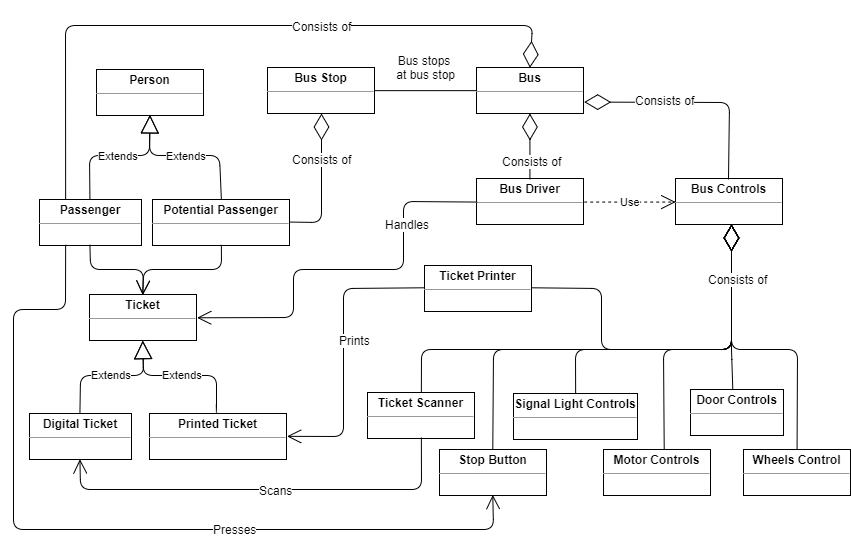
\includegraphics[scale=0.49]{Images/problem_domain_class_diagram.png}
\caption{Class diagram for the problem domain.}
\label{problem-domain-class-diagram}
\end{figure}


\subsection{Behaviour pattern}

Since the central part of the project aims to replace the bus driver, the persons behaviour is relevant to our project. This is  

\begin{figure}[H]
\centering
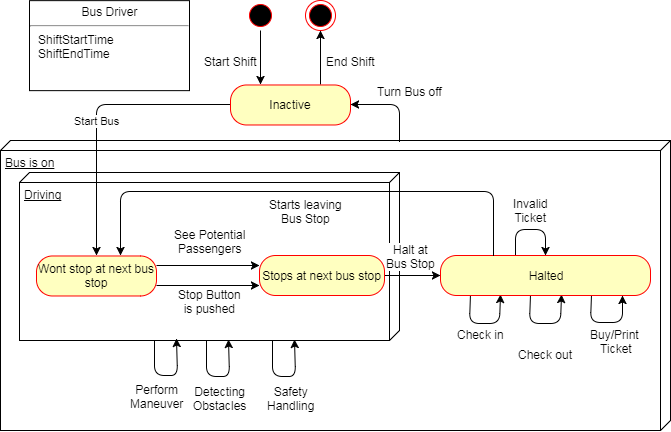
\includegraphics[scale=0.6]{Images/BehaviorDiagramBusDriver.png}
\caption{Behaviour diagram for the bus driver.}
\label{BehaviorDiagramBusDriver}
\end{figure}